\chapter{Inverted Indexes\label{invindex}}

Most of the information present in this chapter is thanks to Mahapatra and Biswas "Inverted indexes: Tyoes and techniques" \citep{fromDocToIndex}. 

What we will need for the algorithms presented in the rest of this documents are inverted indexes (also called posting lists). To get them we first need to process documents into lists of words (called \textit{word tokens}), then for each token compute a list of \verb+IDs+ that refer to the documents which contain that specific token. Let's see each step in order.

\section{Document Pre-Processing}

Documents go trough a series of processing steps before being indexed: they get converted into token in the lexing phase, which are then possibly normalized, stemmed or even pruned (removed) entirely.

\subsection{Lexing}

\begin{wrapfigure}{r}{0.5\textwidth} %this figure will be at the right
    \centering
    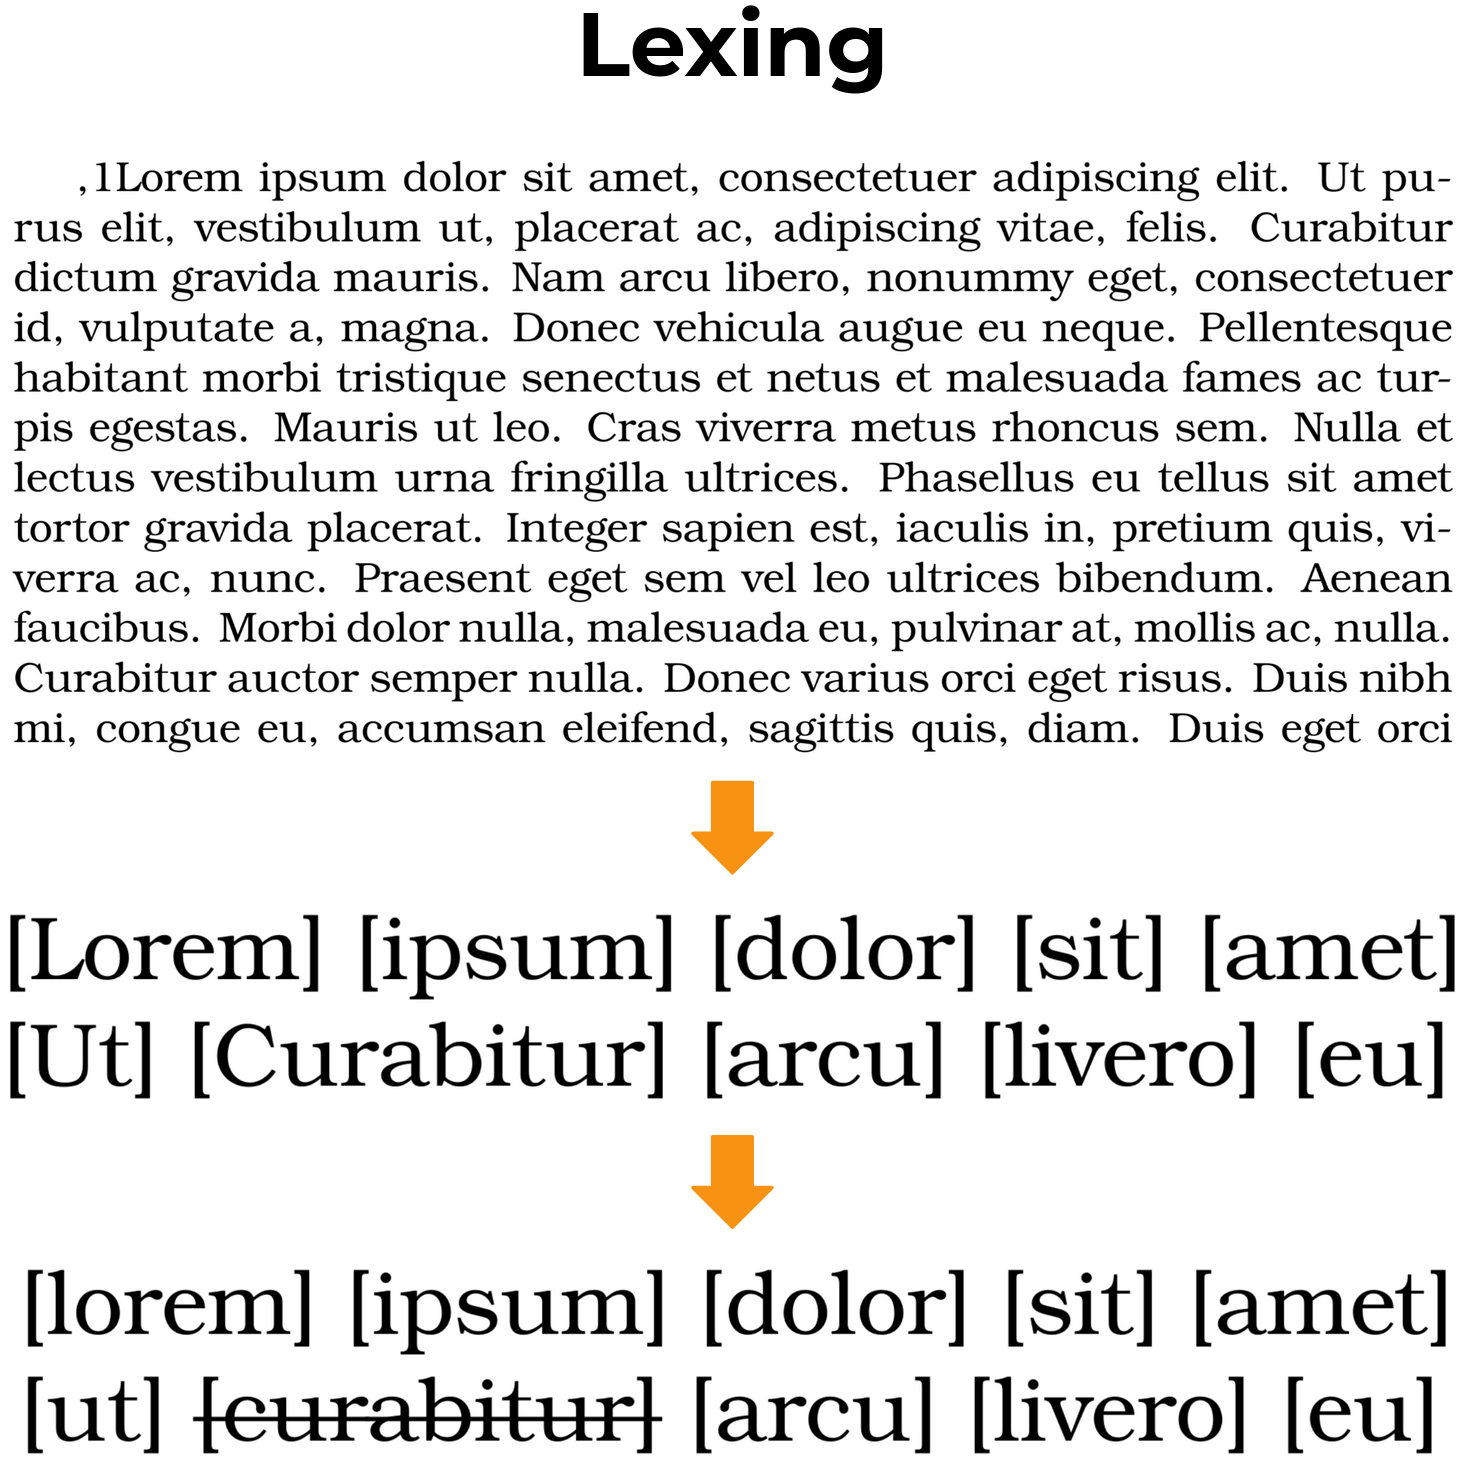
\includegraphics[width=.5\textwidth]{imgs/lorem_lexing.png}
    \caption{Lexing: from text to word tokens\label{fig:lorem_lexing}}
\end{wrapfigure}

The process of transforming a document into a list of tokens, each of which is a single word, si called \textit{lexing} [\ref{fig:lorem_lexing}]. There often is a maximum length for a single token, as to prevent unbounded index growth in edge cases, and all input is generally first converted into lower-case to normalize it. The all non-punctuation characters are added to the list of tokens one by one, and those that exceed a certain size are often pruned (removed from the corpus). It is not entirely clear how Google and other big companies do this step, and it certainly feels strange to think they employ a simple \textit{brute force}, single scan approach, but as mentioned before it is not easy to find information about it. \\
All of the above works only with alphabetic languages, ideographic ones (e.g., Chinese) need specialized search techniques. 

\subsection{Stemming}

